\documentclass[accentcolor=tud6b,11pt,paper=a4]{tudreport}

\usepackage[T1]{fontenc} 
\usepackage[utf8]{inputenc} 
\usepackage[ngerman]{babel}
\usepackage{listings}
\usepackage{pdfpages}

%======================================================
% KOM-modifications of the TUD-layout
%======================================================
% reduce font size of page footers and headers (fancyhdr)
\renewcommand{\footerfont}{\fontfamily{\sfdefault}\fontseries{m}\fontshape{n}\footnotesize\selectfont}
% remove space between items 
\usepackage{enumitem}
	\setenumerate{noitemsep}
	\setitemize{noitemsep}
	\setdescription{noitemsep}
%\setlist{nolistsep}

%======================================================
% Package loading for example contents (content.tex)
%======================================================
\usepackage{tabularx} % better tables
\setlength{\extrarowheight}{3pt} % increase table row height
\usepackage{booktabs}
\usepackage{caption}
\captionsetup{format=hang,font=small}
\usepackage[square,numbers]{natbib}
\usepackage{subfig}
\usepackage[stable,bottom]{footmisc}

%======================================================
% Setup for hyperref
%======================================================
\usepackage[pdftex,hyperfootnotes=true,pdfpagelabels]{hyperref}
\pdfcompresslevel=9
\pdfadjustspacing=1 
\hypersetup{
    pdftitle={XGVisualize, Ausarbeitung},%
    pdfauthor={Michael Br\"aunleinr, DKE, TU Darmstadt}
}

%============================================
% Setup of the title page (do not change)
%============================================
\title{Klassifikation der Schwierigkeitsgrade von Sudokus mit Methoden des maschinellen Lernens}
\subtitle{Investigation of Sudoku difficulty levels}
\subsubtitle{Bachelor-Thesis von Michael Br\"aunlein}
\institution{\raggedleft Fachbereich Informatik \\
	Knowledge Engineering Group
	Betreuer Prof. Dr. Johannes F\"urnkranz
}
	
\begin{document}

\maketitle

% ===== abstract ==========================================
\begin{abstract}
Das Zahlenr\"atsel Sudoku ist weltweit bei R\"atselliebhabern bekannt und beliebt. Seit seiner Ver\"offentlicheung 1986 begeistern sich immer mehr Menschen f\"ur mehr oder weniger schwierige Exemplare. Sudokus finden sich im Internet, in der R\"atselecke der Tageszeitungen und sogar als ganze B\"ucher, um nur einige Erscheinungsorte zu nennen. \\
Die Regeln sind einfach zu lernen und doch kann man sich sehr lange mit Sudokus besch\"aftigen, da die schwersten Sudokus meißt nur von Profis gel\"ost werden k\"onnen.\\
Der Spielspass ist sehr stark davon abh\"angig, dass die Schwierigkeit zum pers\"onlichen K\"onnen passt. Ist das Sudoku zu leicht, stellt es keine Herausforderung dar. Ist es zu schwer, kommt schnell ein Gef\"uhl der \"Uberforderung auf. \\
Die ausgewiesenen Schwierigkeitsstufen von Sudokus aus verschiedenen Quellen haben zwar of die gleeichen Namen wie zum Beispiel 
\textquotedblleft Mittel\textquotedblright
, unterscheiden sich aber dennoch h\"aufig nach Meinung des Spielers.\\
Das Ziel dieser Bachelorarbeit ist, Merkmale aus Sudokus zu extrahieren, anhand derer die Sudokus von einem Klassifizierer m\"oglichst zuverl\"assig in Schwierigkeitsstufen eingeteilt werden k\"onnen.\\
\end{abstract}

% ===== lists =============================================
\tableofcontents

\chapter{Aufgabenstellung und Zielsetzung}
Diese Bachelorarbeit besch\"aftigt sich mit der Einteilung von Sudokus in verschiedene Schwierigkeitsstufen. Hierzu sollen Methoden des maschinellen Lernens verwendet werden. \\ Es soll eine Methode gefunden werden, mit der Merkmale aus Sudokus extrahiert werden können, die dann als Feature Vectoren in einer .arff Datei\footnote{\url{http://www.cs.waikato.ac.nz/ml/weka/arff.html}} gesammelt werden. Die Feature Vectoren werden anschließend mit Hilfe von Weka\footnote{\url{http://www.cs.waikato.ac.nz/ml/weka/}} klassifiziert.\\
Es werden verschiedene Klassifikatoren und unterschiedliche Parameter betrachtet. Ausserdem werden Optimierungen der Featurevektoren diskutiert.


%======================================================

\chapter{Einf\"uhrung}
Die Vorfahren des heutigen Sudokus waren vermutlich die lateinischen Quadrate, mit denen sich vor allem der Mathematiker Leonhard Euler befasste. Hier ging es darum, in ein Quadrat mit n Spalten und n Reihen Symbole so einzutragen, dass jedes Symbol in jeder Spalte und Zeile jeweils genau einmal vorkommt.

\begin{figure}[htbp]
\begin{center}
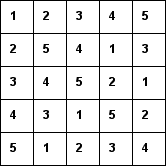
\includegraphics{./img/lat_quadrat.png}
\caption{Lateinisches Quadtrat}
\end{center}
\end{figure}

Daraus hat sich das heutige Sudoku entwickelt, das sich nicht nur bei Mathematikern großer Beliebtheit erfreut.

\section{Die Regeln}
Diese Arbeit besch\"aftigt sich nur mit der meist verbreiteten Art von Sudokus. Dabei spielt man auf einem 9x9 Felder großen Spielfeld, das wiederum in neun 3x3 Felder große Bl\"ocke eingeteilt ist. Weiter handelt es sich nur dann um ein Sudoku, wenn genau eine L\"osung vorhanden ist.
Ein Sudoku gilt dann als gel\"ost, wenn jede Zeile, jede Spalte und jeder Block die Ziffern 1 bis 9 genau einmal enth\"alt.\\
\begin{figure}[h]
\begin{center}
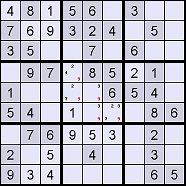
\includegraphics{./img/sudoku.jpg}
\caption{Sudoku}
\end{center}
\end{figure}


\section{Begriffserklärung}
Ein Sudoku besteht aus 81 \textit{Feldern} oder \textit{Zellen}. Diese bilden ein Quadrat der Gr\"oße 9x9, das \textit{Grid}. Aufgrund dieser Aufteilung hat ein Sudoku 9 \textit{Zeilen} und 9 \textit{Spalten}. Das Grid wird in 9 Unterquadrate geteilt, die jeweils 3x3 Felder groß sind. Diese werden \textit{Bl\"ocke} genannt. Zeilen, Spalten und Bl\"ocke werden unter dem Begriff \textit{Figur} zusammengfasst. Die Nummerierung der Bl\"ocke erfolgt zeilenweise von links oben nach rechts unten.\\
\textit{Vorgaben} sind Zahlen, die schon von Anfang an gegeben sind.\\
In \textbf{Abbildung 2.2} sieht man im mittleren Block sogenannte \textit{Kandidaten}. Ein Kandidat ist eine Zahl, die in der Zelle noch m\"oglich ist. Jede Zelle hat ihre eigene Liste mit Kandidaten.\\
In der Beschreibung der L\"osungstechniken ist es notwendig bestimmte Felder zu betrachten. Hierzu wird eine Abk\"urzung verwendet, die Zeile und Spalte enth\"alt und somit eine Zelle eindeutig indentifiziert. \textit{z2s3} meint zum Beispiel die Zelle in Zeile 2 und Spalte 3.\\
In der folgenden Abbildung sind die erl\"auterten Begriffe zum besseren Verst\"andniss eingetragen.\\

\begin{figure}[h]
\begin{center}
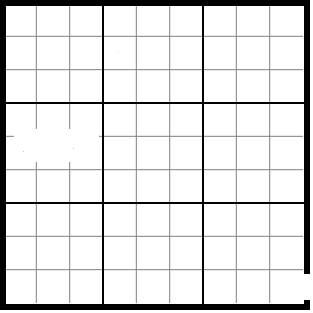
\includegraphics{./img/begriffe.png}
\caption{Begriffe}
\end{center}
\end{figure}
%======================================================

\chapter{L\"osungsmethoden}
Alle in dieser Bachelorarbeit beschriebenen Techniken sind nicht im Rahmen dieser Arbeit entwickelt worden, sondern wurden aus verschiedenen Quellen zusammengetragen. Die Beschreibung der L\"osungstechniken lehnt sich an die Beschreibung der Quellen an. Teile der Beispiele wurden aus den Quellen entnommen, dies ist entsprechend gekennzeichnet.\\
Grob kann man die Techniken zum L\"osen von Sudokus in zwei Kategorien einteilen. Die erste Kategorie findet Zahlen heraus, die direkt in das Sudoku eingetragen werden k\"onnen. Die Techniken der zweiten Kategorie entfernen Bedingungen in einzelnen Zellen des Sudokus.

\section{Kandidatenlisten}
Beim L\"osen von Sudokus ist es \"ublich, in jedes Feld die Kandidaten einzutragen, die dort stehen k\"onnen. Dabei wird vorerst nur die Sudoku Regel ber\"ucksichtigt, die besagt, dass in jeder Figure die Zahlen 1 bis 9 vorkommen m\"ussen. Wenn in einer Zeile nun die Zahl 3 vorkommt, dann kann sie in der selben Zeile nicht nochmal vorkommen, daher kann sie aus allen Kandidatenlisten der Zellen in der selben Zeile gel\"oscht werden. Dasselbe gilt f\"ur Spalten und Bl\"ocke. Immer wenn eine Ziffer in ein Feld eingetragen wird, dann muss der Spieler die Liste der Kandidaten aktualisieren.\\
Kandidatenlisten sind keine eigene L\"osungstechnik, sind aber wesentlicher Bestandteil vieler Techniken.

\newpage
\section{Full House}
Wenn in einer Figur 8 Zahlen eingetragen sind, dann kann die Technik \textit{Full House} angewendet werden. Da in jeder Figur die Zahlen 1 bis 9 stehen m\"ussen, kann die fehlende Zahl einfach per Ausschluss ermittelt werden.\\
Im folgenden Beispiel fehlt in Zeile 5 nur noch eine Ziffer. Da die Zahlen 2 bis 9 bereits vorhanden sind, kann in das Feld z5s8 die Zahl 1 eingetragen werden.

\begin{figure}[h]
\begin{center}
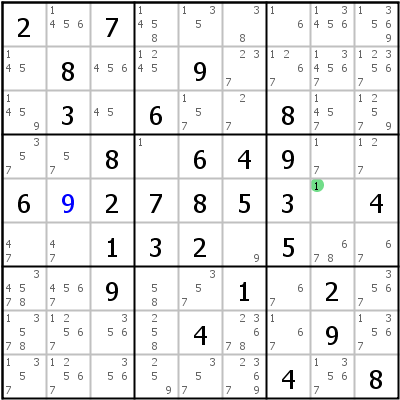
\includegraphics{./img/fullhouse.png}
\caption{Full House}
\end{center}
\end{figure}

\newpage
\section{Naked Single}

\section{Hidden Single}
\section{Pointing Pair / Triple}
\section{Box-Line Reduction}
\section{Naked Subset}
\section{Hidden Subset}
\section{Fish}
\subsection{X-Wing}
\subsection{Swordfish}
\subsection{Jellyfish}
\section{Single Digit Patterns}
\subsection{Skyscarper}
\subsection{2-String Kite}
\subsection{Turbot Fish}
\subsection{Empty Rectangle}
\section{Wings}
\subsection{XY-Wing}
\subsection{XYZ-Wing}
\subsection{W-Wing}
\section{Sue de Coq}
\section{Coloring}
\section{Almost Locked Set}
\subsection{ALS XZ}
\subsection{ALS XY Wing}
\subsection{ALS Chain}

%======================================================

\chapter{Merkmalsextrahierung}
\section{Allgemeines Vorgehen}
\section{Entkopplung von konkreten Zahlen}
%======================================================

\end{document}